\subsection{Описание системы стереозрения}

Предлагаемая система стереозрения состоит из двух или более камер с объективами типа "рыбий глаз" $>=180\deg$,
расположенных своими оптическими осями под некоторым углом. В таком случае поля зрения камер попарно пересекаются, 
образуя  область, точки пространства в которой видны на обеих камерах. Это позволяет получить информацию о 
глубине в указанной области.
                            % FIXME: Всё описание просто бггг
Для успешной реализации алгоритма стереозрения в каждой камере создаются виртуальные камеры-обскуры, направленные 
своими оптическими осями параллельно биссектрисе угла, образованного пересечением полей зрения fisheye-камер. Количество
 виртуальных камер для каждой реальной в общем случае равно количеству соседних реальных камер с пересекающимися полями 
 зрения. Пример такой системы для робота "Капитан" представлен на рисунке \ref{pic:4cam_system}. Здесь 4 камеры, изображённых
 полукругами, с центрами в точках $C_{0-3}$ размещены спереди, сзади и по бортам корпуса робота. Пересечения их полей зрения 
 образуют 4 области объёмного зрения, закрашенных голубым.    % TODO: дополнить описание картинки (и нарисовать саму картинку) 
 \begin{figure}[H]
    \begin{center}
        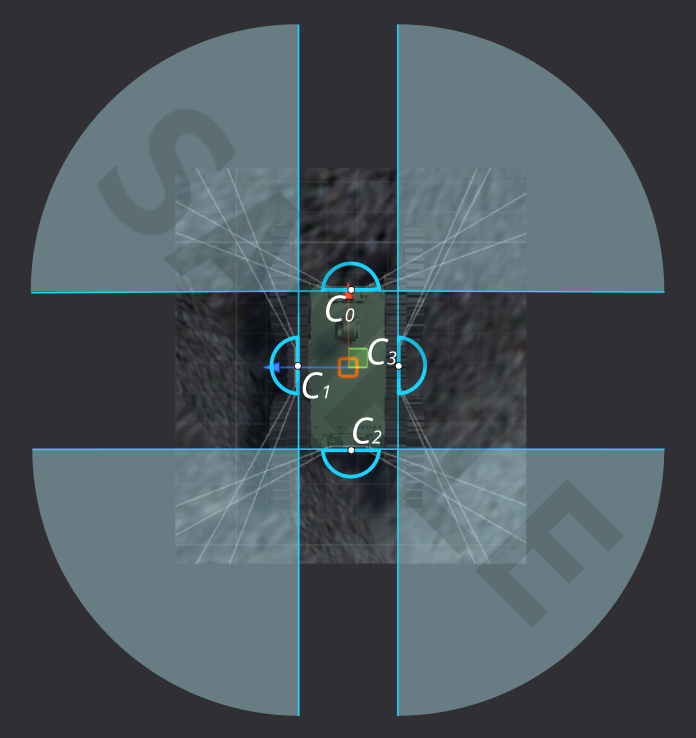
\includegraphics[scale=0.5]{pics/sample_4cam.png}                                                               %TODO: перерисовать схему?
        \caption{Система стереозрения на основе четырёх камер на примере робота "Капитан"}
        \label{pic:4cam_system}
    \end{center}
\end{figure}
 Далее для примера рассмотрим вариант системы с двумя камерами под углом $90\deg$, соответствующий фрагменту схемы,     % FIXME: не совсем соответствует теперь
  представленной на рисунке \ref{pic:4cam_system}. Здесь ... % TODO: пояснить обозначения
\begin{figure}[H]
    \begin{center}
        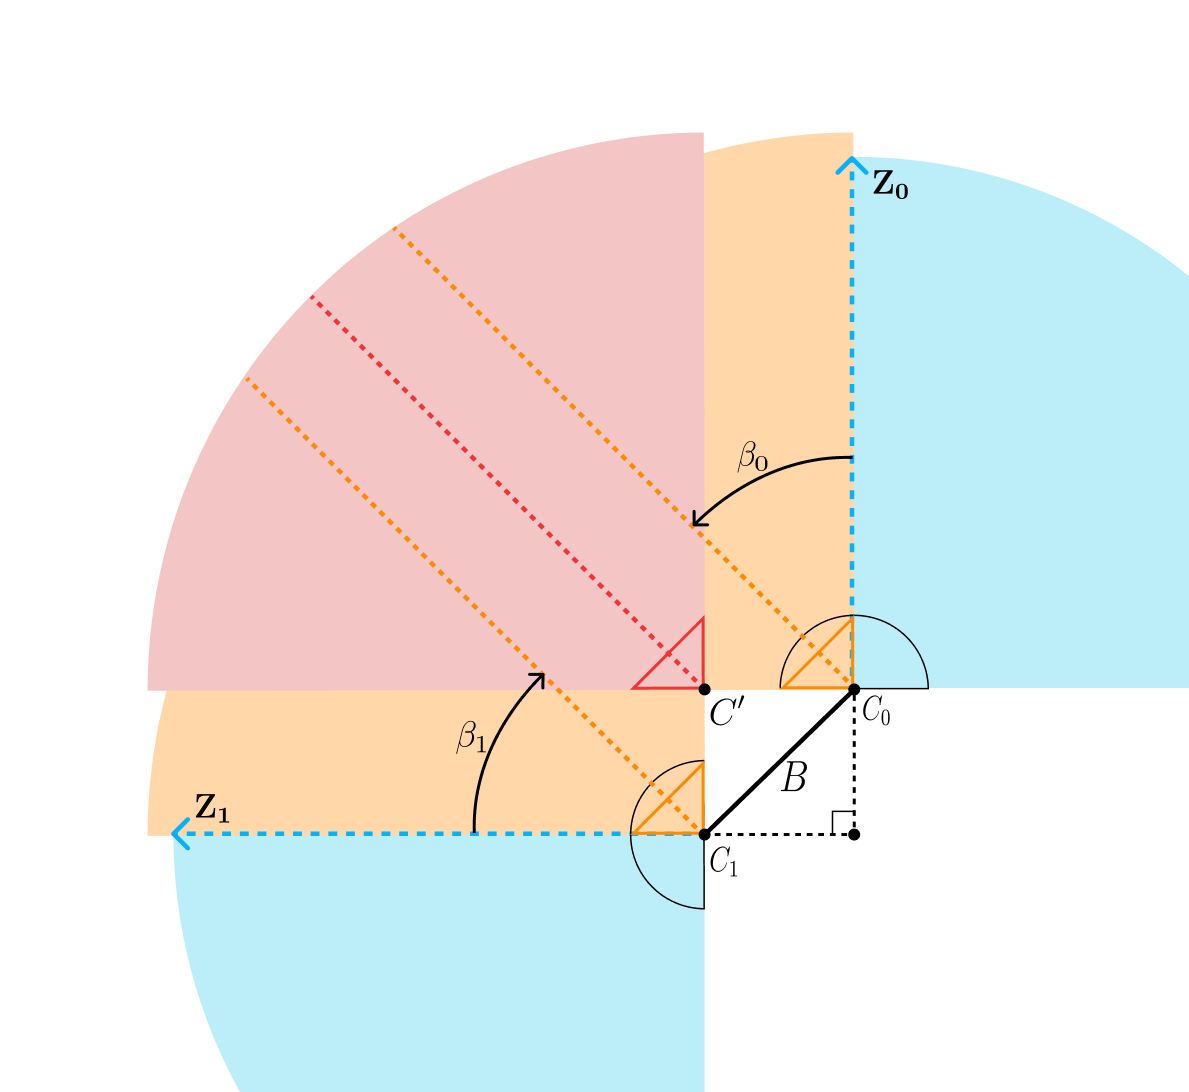
\includegraphics[scale=0.5]{pics/sample_simple2cam.png}                                                          %TODO: перерисовать схему?
        \caption{Геометрическая модель бинокулярной системы стереозрения}
        \label{pic:2cam_scheme}
    \end{center}
\end{figure}
